\documentclass{zusammenfassung}
\graphicspath{ {./illustrationen/} }

\usetikzlibrary{knots}

\begin{document}
\maketitle{Klasse 6/7}{18. November 2014}{2014/2015}

Ein \emph{mathematischer Knoten} ist eine geschlossene Kurve im Raum. Es ist also wichtig, dass der Knoten
\begin{itemize}
  \item keine losen Enden hat,
  \item nur aus einem Stück (einer \emph{Komponente}) besteht und
  \item es keine Verzweigungen gibt.
\end{itemize}

\begin{aufgabe}[Beispiele und Nichtbeispiele von Knoten]
  \label{aufgabe1}
  Welches der Bilder zeigt einen (mathematischen) Knoten?\\[0.5ex]

\begin{tikzpicture}[every path/.style={black, ultra thick}]
  \node[anchor=north west] at (-2,3) {a)};
  \begin{knot}[
%      draft mode=strands,
%      draft mode=crossings,
      consider self intersections,
      end tolerance=0.1,
      clip width=5,
      flip crossing/.list={2}
    ]
    \strand (0,0) ..controls (0.5,0) and (1,0.2)..
    	    (1,0.5) ..controls (1,1) and (0,1)..
            (0,1.5) ..controls (0,2) and (1,2)..
            (1,2.5) ..controls (1,2.8) and (0.5,3)..
            (0,3) ..controls (-0.5,3) and (-1,2.5)..
            (-1,2) ..controls (-1,1.5) and (-0.5,1)..
            (0,1) ..controls (0.3,1) and (0.5,1.2)..
            (0.5,1.5) ..controls (0.5,1.8) and (0.3,2)..
            (0,2) ..controls (-0.5,2) and (-1,1.5)..
            (-1,1) ..controls (-1,0.5) and (-0.5,0)..
            (0,0);

  \end{knot}
  \node[anchor=north west] at (2,3) {b)};
  \begin{knot}[
%      draft mode=strands,
%      draft mode=crossings,
      consider self intersections,
      end tolerance=0.1,
      clip width=5,
      flip crossing/.list={2}
    ]
    \strand (2.8,1) ..controls (3.5,1) and (3.5,1.5)..
            (4,1.5) ..controls (4.5,1.5) and (4.5,1)..
	    (5,1) ..controls (5.2,1) and (5.5,1.2)..
	    (5.5,1.5) ..controls (5.5,1.8) and (5,2.2)..
	    (4.5,2.2) ..controls (4,2.2) and (3.5,1.8)..
	    (3.5,1.5) ..controls (3.5,1.2) and (3.8,1)..
	    (4,1) ..controls (4.5,1) and (4.5,1.5)..
	    (5,1.5) ..controls (5.5,1.5) and (5.5,1)..
	    (6.2,1);
  \end{knot}
  \node[anchor=north west] at (7,3) {c)};
  \draw (9,1.5) circle (1);
  \node[anchor=north west] at (-2,-1) {d)};
  \begin{knot}[
%      draft mode=strands,
%      draft mode=crossings,
      consider self intersections,
      end tolerance=0.1,
      clip width=5,
      flip crossing/.list={2}
    ]
    \strand (-0.5,-2.5) circle (0.8) (0.5,-2.5) circle (0.8);
  \end{knot}
  \node[anchor=north west] at (2,-1) {e)};
  \draw (4,-2.5) circle (1);
  \draw[shift={(4,-2.5)}] (320:1) ..controls (1.5,-1) and (2,-0.5)..
  			  (2,0) ..controls (2,0.5) and (1.5,1).. (40:1);
  \fill[shift={(4,-2.5)}] (320:1) circle (0.1) (40:1) circle (0.1);
\end{tikzpicture}
\end{aufgabe}

Von den Bildern in Aufgabe \ref{aufgabe1} zeigen nur a) und c) mathematische Knoten: Bei b) ist die Kurve nicht geschlossen, das 
Bild aus d) hat mehr als eine Komponente, und bei e) gibt es Verzweigungen, die nicht erlaubt sind. Der Knoten aus c) ist der
einfachste Knoten, den es gibt; er heißt \emph{Unknoten.}

Man kann sich jetzt die Frage stellen, wann zwei Knoten "`gleich"' sind. Ein sinnvoller Ansatz ist dabei, dass man zwei Knoten
\emph{äquivalent} nennt, wenn man sie (ohne eine Schere und Kleber zu benutzen) ineinander umformen kann. Dabei sollte man sich
die Knoten aus sehr gut dehnbarem Gummi gefertigt vorstellen.

Um das besser modellieren zu können, kann man sich die Knoten auch als Vielecke im Raum vorstellen. Ein Knoten besteht also aus
aneinandergefügten Stäben von unterschiedlicher Länge wie in folgendem Bild:

\begin{center}
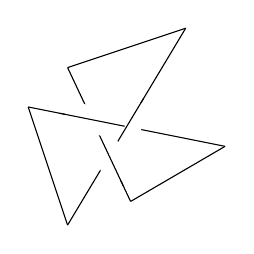
\begin{tikzpicture}[%every path/.style={black,thick}, 
  x=1cm, y=1cm]
  \begin{knot}[
%      draft mode=crossings,
      ignore endpoint intersections,
      clip width=5,
    ]
    \strand (0,0) -- (1.5,0.5);
    \strand (1.5,0.5) -- (0,-2);
    \strand (0,-2) -- (-0.5,-0.5);
    \strand (-0.5,-0.5) -- (2,-1);
    \strand (2,-1) -- (0.8,-1.7);
    \strand (0.8,-1.7) -- (0,0);
    \flipcrossings{2}
  \end{knot}
\end{tikzpicture}
\end{center}

In diesem Modell sind dann folgende Bewegungen möglich:

\begin{center}
  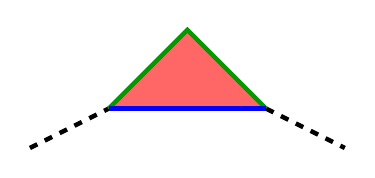
\begin{tikzpicture}[every path/.style={ultra thick}]
    \draw[dashed] (0,0.5)--(1,1);
    \draw[dashed] (3,1)--(4,0.5);
    \fill[red!60!white] (1,1)--(2,2)--(3,1)--cycle;
    \draw[green!60!black] (1,1)--(2,2)--(3,1);
    \draw[blue] (1,1)--(3,1);
  \end{tikzpicture}
\end{center}

Wenn durch das rote Dreieck kein anderer Stab des Knotens geht, dann darf der grüne Teil durch den blauen ersetzt werden, und man
erhält einen äquivalenten Knoten. Im Jahr 1926 bewies der deutsche Mathematiker Kurt Reidemeister mit Hilfe von vielen
Fallunterscheidungen, dass sich jede Bewegung wie im Bild oben aus einfachen Bewegungen zusammensetzen lässt, den sogenannten
\emph{Reidemeister-Bewegungen.}

Es gibt drei Typen von Reidemeister-Bewegungen:
\begin{itemize}
  \item Typ I erlaubt es, Schlaufen in ein Stück des Knotens einzufügen oder sie zu lösen,
  \item Typ II lässt es zu, zwei Seilstücke untereinander vorbeizuschieben und
  \item Typ III erlaubt es, ein Seilstück an einer Kreuzung vorbeizubewegen.
\end{itemize}

\begin{center}
\begin{tikzpicture}[every path/.style={ultra thick},y=0.9cm]
  \draw (11.5,0)--(11.5,3);
  \node[anchor=center] at (12.5,1.5) {\scalebox{1.5}{$\leftrightsquigarrow$}};
  \node[anchor=center] at (12.5,2) {Typ I};
  \begin{knot}[
%      draft mode=strands,
%      draft mode=crossings,
      consider self intersections,
      end tolerance=0.1,
      clip width=5,
      flip crossing/.list={2}
    ]
    \strand (13.5,0) ..controls (13.4,1) and (13.7,1.8)..
            (14,1.8) ..controls (14.2,1.8) and (14.3,1.7)..
            (14.3,1.5) ..controls (14.3,1.3) and (14.2,1.2)..
	    (14,1.2) ..controls (13.7,1.2) and (13.4,2)..
	    (13.5,3);
  \end{knot}
  \draw (16.5,0)--(16.5,3);
  \draw (17.5,0)--(17.5,3);
  \node[anchor=center] at (18.5,1.5) {\scalebox{1.5}{$\leftrightsquigarrow$}};
  \node[anchor=center] at (18.5,2) {Typ II};
  \begin{knot}[
%      draft mode=strands,
%      draft mode=crossings,
      clip width=5,
    ]
    \strand (19.5,0) ..controls (19.5,0.5) and (21,1)..
    	    (21,1.5) ..controls (21,2) and (19.5,2.5)..
	    (19.5,3);
    \strand (20.5,0)--(20.5,3);
  \end{knot}
  \begin{scope}[shift={(1,0)}]
  \begin{knot}[
%      draft mode=crossings,
      clip width=5
    ]
    \strand (12,-4) -- (14,-1);
    \strand (14,-4) -- (12,-1);
    \strand (12.7,-4) -- (12.7,-1);
  \end{knot}
  \node[anchor=center] at (15,-2.5) {\scalebox{1.5}{$\leftrightsquigarrow$}};
  \node[anchor=center] at (15,-2) {Typ III};
  \begin{knot}[
%      draft mode=crossings,
      clip width=5
    ]
    \strand (16,-4) -- (18,-1);
    \strand (18,-4) -- (16,-1);
    \strand (16.7,-4) ..controls (16.7,-3.5) and (17.3,-3.5) ..
    	    (17.3,-2.5) ..controls (17.3,-1.5) and (16.7,-1.5) ..
	    (16.7,-1);
  \end{knot}
  \end{scope}
\end{tikzpicture}
\end{center}

Den Satz von Reidemeister kann man also folgendermaßen formulieren: \emph{Zwei Knoten sind genau dann äquivalent, wenn man sie mit
(beliebig vielen) Reidemeister-Bewegungen ineinander überführen kann.}

\begin{aufgabe}[Reidemeister-Bewegungen]
  Wie lassen sich die folgenden Bewegungen aus Reidemeister-Bewegungen zusammensetzen?\\[0.5ex]

\begin{tikzpicture}[every path/.style={black,ultra thick}, x=1cm, y=-1cm]
  \node[anchor=north west] at (0,0) {a)};
  \begin{knot}[
%      draft mode=strands,
%      draft mode=crossings,
      consider self intersections,
      end tolerance=0.1,
      clip width=5,
%      flip crossing/.list={2}
    ]
    \strand (1,0) ..controls (1.5,0.5) and (2,1)..
            (2,1.5) ..controls (2,2) and (1.5,2.5)..
	    (1,3);
    \strand (2.5,0) ..controls (2,0.5) and (1.5,1)..
            (1.5,1.5) ..controls (1.5,2) and (2,2.5)..
	    (2.5,3);
  \end{knot}
  \node[anchor=center] at (3,1.5) {\scalebox{1.5}{$\leftrightsquigarrow$}};
  \draw (4,0) -- (4,3) (5,0) -- (5,3);
  \node[anchor=north west] at (6,0) {b)};
  \begin{knot}[
%      draft mode=strands,
%      draft mode=crossings,
      consider self intersections,
      end tolerance=0.1,
      clip width=5,
      flip crossing/.list={2,3}
    ]
    \strand[shift={(0.7,0)}] (7,0) ..controls (7.7,0.8) and (8,2)..
            (8.5,2) ..controls (8.8,2) and (9,1.7)..
	    (9,1.5) ..controls (9,1.3) and (8.8,1)..
	    (8.5,1) ..controls (8,1) and (7.7,2.2)..
	    (7,3);
    \strand (9,0) ..controls (8.3,0.8) and (8,2)..
            (7.5,2) ..controls (7.2,2) and (7,1.7)..
	    (7,1.5) ..controls (7,1.3) and (7.2,1)..
	    (7.5,1) ..controls (8,1) and (8.3,2.2)..
	    (9,3);
  \end{knot}
  \node[anchor=center] at (10.5,1.5) {\scalebox{1.5}{$\leftrightsquigarrow$}};
  \begin{knot}[
%      draft mode=strands,
%      draft mode=crossings,
      consider self intersections,
      end tolerance=0.1,
      clip width=5,
      flip crossing/.list={2}
    ]
    \strand (12.5,0) ..controls (12.6,1) and (12.3,1.8)..
            (12,1.8) ..controls (11.8,1.8) and (11.7,1.7)..
            (11.7,1.5) ..controls (11.7,1.3) and (11.8,1.2)..
	    (12,1.2) ..controls (12.3,1.2) and (12.6,2)..
	    (12.5,3);
    \strand (13.5,0) ..controls (13.4,1) and (13.7,1.8)..
            (14,1.8) ..controls (14.2,1.8) and (14.3,1.7)..
            (14.3,1.5) ..controls (14.3,1.3) and (14.2,1.2)..
	    (14,1.2) ..controls (13.7,1.2) and (13.4,2)..
	    (13.5,3);
  \end{knot}
\end{tikzpicture}
\end{aufgabe}

Bei Teil a) ist eine Typ-II-Reidemeister-Bewegung nur etwas verändert angegeben, bei Teil b) müssen zuerst die Schlaufen mit Typ I
gelöst, dann die Seilstücke mit Typ II aneinander vorbeibewegt und die Schlaufen mit Typ I wieder eingefügt werden.

Ein wichtiges Ziel ist es zu zeigen, dass es verschiedene nicht äquivalente Knoten gibt. Dazu führt man den Begriff der
\emph{Dreifärbbarkeit} ein: Eine Knotenprojektion heißt \emph{dreifärbbar,} wenn man sie mit drei verschiedenen Farben so
einfärben kann, dass
\begin{itemize}
  \item die Farben auf jedem zusammenhängend sichtbaren Stück der Projektion gleich bleiben und
  \item an jeder Kreuzung entweder eine oder drei verschiedene Farben zusammenkommen, aber nie zwei.
\end{itemize}

Beispielsweise ist der sogenannte Kleeblattknoten dreifärbbar:

\begin{center}
  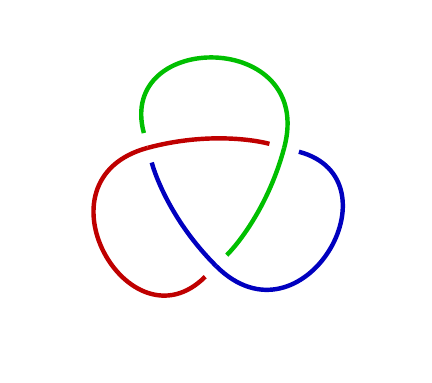
\begin{tikzpicture}[every path/.style={black,ultra thick}, every node/.style={transform shape, knot crossing}]
    \node[rotate=150] (tl) at (150:1) {};
    \node[rotate=30] (tr) at (30:1) {};
    \node[rotate=270] (b) at (270:1) {};
    \draw[red!75!black] (tr) ..controls (tr.2 north west) and (tl.4 south west).. (tl.center);
    \draw[red!75!black] (tl.center) ..controls (tl.8 north east) and (b.8 south east).. (b);
    \draw[blue!75!black] (tl) ..controls (tl.2 north west) and (b.4 south west).. (b.center);
    \draw[blue!75!black] (b.center) ..controls (b.8 north east) and (tr.8 south east).. (tr);
    \draw[green!75!black] (b) ..controls (b.2 north west) and (tr.4 south west).. (tr.center);
    \draw[green!75!black] (tr.center) ..controls (tr.8 north east) and (tl.8 south east).. (tl);
  \end{tikzpicture}
\end{center}

Offensichtlich ist der Unknoten allerdings nicht dreifärbbar, denn er besteht ja nur aus einem zusammenhängenden Stück. Man kann
sich nun überlegen, dass die Reidemeister-Be\-we\-gun\-gen nichts an der Dreifärbbarkeit ändern:
\begin{itemize}
  \item Bei Typ I muss vor der Bewegung das ganze Teilstück (mit oder ohne Schlaufe) in derselben Farbe eingefärbt sein.
  \item Bei Typ II können entweder beider Stränge dieselbe Farbe oder unterschiedliche Farben haben. Im letzteren Fall muss man
    das überdeckte Teilstück einfach in der dritten verfügbaren Farbe einfärben. 
  \item Ähnlich kann man mit ein paar Fallunterscheidungen zeigen, dass auch Typ-III-Rei\-de\-mei\-ster-Bewegungen die 
    Dreifärbbarkeit nicht zerstören.
\end{itemize}

Zusammenfassend lässt sich mit Hilfe des Satzes von Reidemeister also sagen: \emph{Entweder alle Projektionen eines Knotens sind
dreifärbbar oder keine ist es.} Da wir eine Projektion des Kleeblattknotens kennen, die dreifärbbar ist, und eine Projektion des
Unknotens, die es nicht ist, haben wir so bewiesen, dass der Kleeblattknoten tatsächlich ein echter Knoten, also nicht äquivalent
zum Unknoten ist.

\begin{aufgabe}[Dreifärbbarkeit von Knoten]
  Ist dieser Knoten dreifärbbar?\\[0.5ex]

  \begin{center}
\begin{tikzpicture}[every path/.style={black,ultra thick},x=1cm,y=-1cm]
%  \node[anchor=north west] at (0,0) {a)};
  \begin{knot}[
%      draft mode=strands,
%      draft mode=crossings,
      consider self intersections,
      end tolerance=0.1,
      clip width=5,
      flip crossing/.list={1,3,5}
    ]
    \strand (1,1.5) ..controls (1,2) and (1.5,2.7)..
            (2,2.7) ..controls (2.4,2.7) and (2.4,3)..
	    (2.8,3) ..controls (3.2,3) and (3.2,2.7)..
	    (3.6,2.7) ..controls (4,2.7) and (4,3)..
	    (4.4,3) ..controls (4.9,3) and (5.4,2)..
	    (5.4,1.5) ..controls (5.4,0.7) and (4.7,0)..
	    (4.1,0) ..controls (3.4,0) and (2.8,0.5)..
	    (2.8,1) ..controls (2.8,1.8) and (4.4,2)..
	    (4.4,2.5) ..controls (4.4,2.8) and (4,3)..
	    (3.6,3) ..controls (3.2,3) and (3.2,2.7)..
	    (2.8,2.7) ..controls (2.4,2.7) and (2.4,3)..
	    (2,3) ..controls (1.8,3) and (1.7,2.8)..
	    (1.7,2.5) ..controls (1.7,2) and (3.6,1.8)..
	    (3.6,1) ..controls (3.6,0.5) and (3,0)..
	    (2.3,0) ..controls (1.7,0) and (1,0.7)..
	    (1,1.5);
  \end{knot}
\end{tikzpicture}
\end{center}
\end{aufgabe}

Hinweis: Die Antwort ist ja.

\end{document}
